\section{Content}

\subsection{Notation}

\begin{Defn}
  \label{defn:1}
  Some definitions, $\cos(x)$ and \(\sin(x)\) are
  \begin{eqnarray}
    \cos(x) \doteq \frac{e^{ix}+e^{-ix}}{2}  \label{eq:fefwe} \\
    \sin(x) \doteq \frac{e^{ix}-e^{-ix}}{2i} \label{eq:fefwe2}
  \end{eqnarray}
  A reference to a figure \ref{fig:a354}.
  A reference \eqref{eq:fefwe} and  \eqref{eq:fefwe2} to the above equations.
\end{Defn}



\begin{figure}[ht]\label{fig:a354}
  \begin{center}
    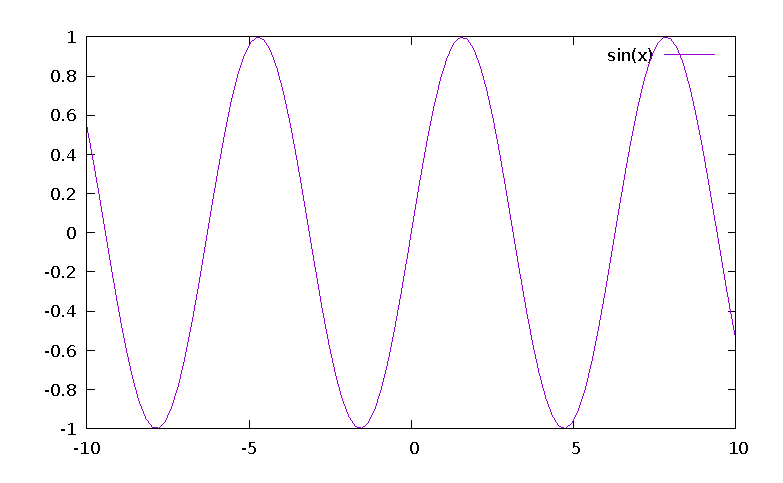
\includegraphics[width=0.5\textwidth]{F/sin}
    \caption{Graph of \(\sin(x)\).}
  \end{center}
\end{figure}


\lipsum[2]


%%% Local Variables:
%%% mode: latex
%%% TeX-master: "book"
%%% End:
